\documentclass{standalone}
\usepackage{tikz}
\usetikzlibrary{positioning, arrows.meta, shapes}
\usetikzlibrary{automata, positioning, arrows,calc}
\usepackage{amsmath}
\begin{document}
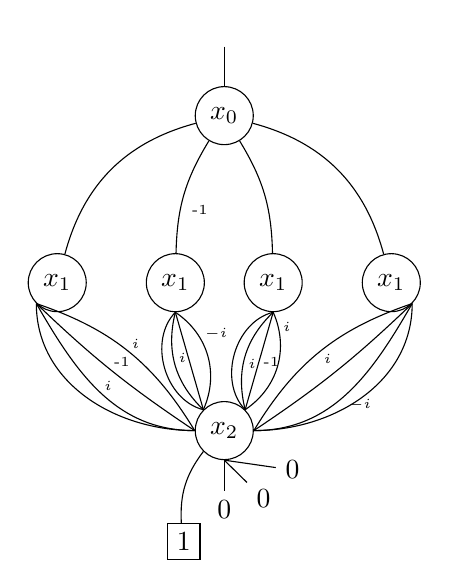
\begin{tikzpicture}[auto, every node/.style={circle, minimum size=0.01cm, align=center}, node distance=2cm,>=Latex]

  % Node styles
  \tikzset{
    state/.style={draw, circle},
    terminal/.style={rectangle}
  }

  % Nodes
  \node[state] (x0) {$x_0$};
  \node[state] (x1_1) at ([shift = ({-135:3cm})]x0) {$x_1$};
  \node[state] (x1_4) at ([shift = ({-45:3cm})]x0) {$x_1$};
  \node[state] (x1_2) at ([shift = ({0:1.5cm})]x1_1) {$x_1$};
  \node[state] (x1_3) at ([shift = ({180:1.5cm})]x1_4) {$x_1$};
  \node[state] (x2) at ([shift = ({-90:4cm})]x0) {$x_2$};
  \node[terminal,draw] (end1) at ([shift = ({-110:1.5cm})]x2) {$1$};
  \node[terminal] (end2) at ([shift = ({-90:1cm})]x2) {$0$};
  \node[terminal] (end3) at ([shift = ({-60:1cm})]x2) {$0$};
  \node[terminal] (end4) at ([shift = ({-30:1cm})]x2) {$0$};
  \node[terminal] (t) at ([shift = ({90:1cm})]x0) {};


  % Edges
%   \draw[->] (x0) -- node[above left] {$-\frac{1}{2}$} (x1_1);
%   \draw[->] (x0) -- node[above right] {$-\frac{1}{2}$} (x1_2);
%   \draw[->] (x1_1) -- node[above left] {$-\frac{1}{2}$} (x2_1);
%   \draw[->] (x1_1) -- node[above right] {$-\frac{1}{2}$} (x2_2);
%   \draw[->] (x2_1) -- (end1);
%   \draw[->] (x2_2) -- (end2);
%   \draw[->] (x1_1) -- node[left] {$-\frac{1}{2}$} (1);
%   \draw[->] (x1_2) -- node[right] {$-\frac{i}{2}$} (1);
%   \draw[->] (x1_1) -- node[left] {$-\frac{i}{2}$} (i);
%   \draw[->] (x1_2) -- node[right] {$-\frac{i}{2}$} (i);
\path[-]
  (x0) edge[bend right=30]  node {} (x1_1)
  (x0) edge[bend right=15]  node[font=\tiny] {-1} (x1_2)
  (x0) edge[bend left=15]  node {} (x1_3)
  (x0) edge[bend left=30]  node {} (x1_4)
  (x1_1.south west) edge[out=-90,in=180] node[inner sep=1pt,font=\tiny] {} (x2.west)
  (x1_1.south west) edge[out=-60,in=180] node[inner sep=1pt,font=\tiny] {$i$} (x2.west)
  (x1_1.south west) edge[bend right=5] node[ inner sep=1pt,font=\tiny] {-1} (x2.west)
  (x1_1.south west) edge[bend left=20] node[ inner sep=1pt,font=\tiny] {$i$} (x2.west)
  (x1_2.south) edge[bend right = 60] node[ inner sep=1pt,font=\tiny] {} (x2.north west)
  (x1_2.south) edge[bend right = 30] node[auto, inner sep=1pt,font=\tiny] {$i$} (x2.north west)
  (x1_2.south) edge[bend left=0] node[auto,inner sep=1pt,font=\tiny] {} (x2.north west)
  (x1_2.south) edge[bend left=40] node[pos=0.4,inner sep=1pt,font=\tiny] {$-i$} (x2.north west)
  (x1_3.south) edge[bend right = 60] node[ inner sep=1pt,font=\tiny] {} (x2.north east)
  (x1_3.south) edge[bend right = 30] node[auto, inner sep=1pt,font=\tiny] {$i$} (x2.north east)
  (x1_3.south) edge[bend left=0] node[pos = 0.4,inner sep=1pt,font=\tiny] {-1} (x2.north east)
  (x1_3.south) edge[bend left=40] node[pos=0.2,inner sep=1pt,font=\tiny] {$i$} (x2.north east)
  (x1_4.south east) edge[out=-90,in=0] node[inner sep=1pt,font=\tiny] {} (x2.east)
  (x1_4.south east) edge[out=-120,in=0] node[pos = 0.5, inner sep=1pt,font=\tiny] {$-i$} (x2.east)
  (x1_4.south east) edge[bend left=5] node[ inner sep=1pt,font=\tiny] {} (x2.east)
  (x1_4.south east) edge[bend right=20] node[ inner sep=1pt,font=\tiny] {$i$} (x2.east)
  ;

  \path[-]
  (x2.south west) edge[bend right=20] node[ inner sep=1pt,font=\tiny] {} (end1)
    (x2.south) edge[] node[ inner sep=1pt,font=\tiny] {} (end2)
  (x2.south) edge[] node[ inner sep=1pt,font=\tiny] {} (end3)
  (x2.south)  edge[] node[ inner sep=1pt,font=\tiny] {} (end4)
  (t)  edge[] node[ inner sep=1pt,font=\tiny] {} (x0)
  ;
\end{tikzpicture}
\end{document}
